\chapter{Διαφορική Ιδιωτικότητα}

Στο προηγούμενο κεφάλαιο αναλύσαμε τεχνικές στις οποίες ο διαχειριστής του συνόλου δεδομένων δημοσιεύει μια εξυγιανσμένη εκδοχή τους. Ωστόσο, είδαμε ότι η ανωνυμοποίηση του συνόλου δεδομένων αρκετές φορές δεν επαρκεί για να προστατέψει τα δεδομένα από έναν ισχυρό και καλά προετοιμασμένο επιτιθέμενο. Σε μια βάση $n$ στοιχείων για παράδειγμα, ένας γνώστης συγκεκριμένου γνωρίσματος των $n-1$ αντικειμένων, μπορεί εύκολα να συμπεράνει την τιμή του γνωρίσματος του ατόμου που απομένει. 
Στη συνέχεια θα παρουσιάσουμε και θα αναλύσουμε την διαφορική ιδιωτικότητα, μια διαδραστική μέθοδο η οποία προστατεύει τα δεδομένα, ακόμη και από επιτιθέμενους με πρότερη γνώση.


\section{Η έννοια της διαδραστικότητας}

\begin{figure} [ht]
\begin{center}
  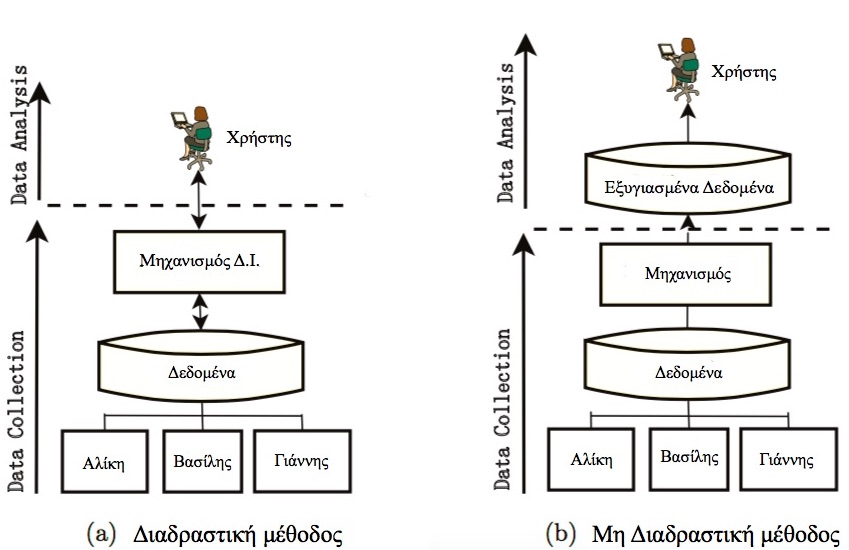
\includegraphics[scale=0.4]{images/Int.jpg}
  \caption{Η έννοια της διαδραστικότητας}
  %\label{fig:boat1}
  \end{center}
\end{figure}
Μία ελπιδοφόρα προσέγγιση που θα μπορούσε να καλύψει τα κενά των τεχνικών ομαδοποίησης που παρουσιάσαμε, είναι να μεσολαβίσει της πρόσβασης στη βάση δεδομένων μια αξιόπιστη διασύνδεση η οποία θα απαντάει τις επερωτήσεις των αναλυτών. 

Έχουν προταθεί κατα καιρούς αρκετές κρυπτογραφικές μέθοδοι, κυρίως μέσω προσθήκης θορύβου, ώστε να διασφαλιστεί η ιδιωτικότητα των μηχανισμών επερωτήσεων και να εξασφαλιστεί η ανώνυμη επικοινωνία Βάσης-Αναλυτή. Σε αυτό το σημείο όμως, είναι εύλογο το ερώτημα:

«Μήπως οι τιμές εξόδου των μηχανισμών αυτών, ήδη αποκαλύπτουν υπερβολικά πολλές πληροφορίες?» 



Μία λύση στο πρόβλημα αυτό είναι η τυχαιοποίηση των αποτελεσμάτων του μηχανισμού.
Υποθέστε ότι κάποιος θέλει να μάθει αν έχουμε  κάποιο συγκεκριμένο χαρακτηριστικό. Σε κάθε τέτοια ερώτηση απαντάμε με τον ακόλουθο τρόπο:

\begin{enumerate}
    \item Ρίχνουμε ένα νόμισμα
    \item Αν έρθει γράμματα, τότε απαντάμε αληθώς.
    \item Αν έρθει κορώνα, τότε ρίχνουμε ένα δεύτερο νόμισμα και απαντάμε «Ναι» αν έρθει κορώνα και «Οχι» αν έρθει γράμματα.
\end{enumerate}

Συμπεραίνουμε ότι δεν μπορεί να προκύψει ακριβές συμπέρασμα για το αν έχουμε ή όχι το χαρακτηριστικό. Αυτό το παράδειγμα παρουσιάζει έναν απλό μηχανισμό τυχαιοποίησης των αποτελεσμάτων των επερωτήσεων. Τον φορμαλισμό της σκέψης  αυτής έρχεται να εκφράσει η διαφορική ιδιωτικότητα.


\section{Θεμελίωση}

Πρωτού δώσουμε τον ορισμό της διαφορικής ιδιωτικότητας θα δούμε δύο ιδιότητες όπου κάθε μέθοδος ιδιωτικότητας οφείλει να κατέχει.

\textbf{Ανθεκτικότητα σε πρότερη γνώση}:

Στο εισαγωγικό παράδειγμα είδαμε ότι υπάρχει πιθανότητα για έναν επιτιθέμενο να έχει γνώση για όλα σχεδόν τα στοιχεία της βάσης. Γενικά οφείλουμε πάντα να λογαριάζουμε οποιαδήποτε πληροφορία μπορεί ήδη να γνωρίζει κάποιος για ένα υποσύνολο δεδομένων. Επειδή είναι πολύ δύσκολο να προσδιοριστεί ποσοτικά, υποθέτουμε ότι ιδανικά ο επιτιθέμενος γνωρίζει τα πάντα, εκτός από τις ατομικές πληροφορίες ενός ατόμου.



\textbf{Ανθεκτικότητα σε πολλαπλές εφαρμογές - Σύνθεση (\textlatin{composition}}):

Αν εφαρμόσουμε την μέθοδο αρκετές φορές σε συγγενείς βάσεις, ο επιτιθέμενος δεν επιτρέπεται να μπορεί να συνδυάσει τα αποτελέσματα ώστε να εξακριβώσει την ταυτότητα κάποιου ατόμου. Εκεί είναι που αποτυγχάνουν οι περισσότερες μη διαδραστικές τεχνικές. Θα αναλύσουμε περισσότερο την ιδιότητα αυτή μετά τον ορισμό της διαφορικής ιδιωτικότητας.




Έστω $x=(x_1,x_2,...,x_n)$ ένα σύνολο δεδομένων, και $x_i$ μια εγγραφή του.

\begin{definition}(Γειτνίαση)\\
Δύο σύνολα δεδομένων $x,x'$ \textbf{γειτνιάζουν}, αν για κάθε στοιχείο τους ισχύει
$ x_i=x'_i $ για κάθε $i\in [1,n]$, εκτός ένός το πολύ στοιχείου.
\end{definition}

Δηλαδή δυο γειτονικά σύνολα δεδομένων πρέπει να διαφέρουν το πολύ σε ένα στοιχείο τους. Συμβολίζουμε $x\sim x'$ 
\textlatin{\cite{dpc}}.

Όταν προτάθηκε για πρώτη φορά διαφορική ιδιωτικότητα , η σχέση γειτνίασης καθορίστηκε με έναν ελαφρώς διαφορετικό τρόπο: δύο βάσεις δεδομένων είναι γειτονικές εάν και μόνο εάν μια βάση δεδομένων είναι αποτέλεσμα της προσθήκης / αφαίρεσης ενός χρήστη από την άλλη βάση δεδομένων\textlatin{\cite{10.1007/11681878_14}}. 

Το κίνητρο πίσω από τον αρχικό ορισμό είναι να γίνει απόκρυψη της συμμετοχής οποιουδήποτε ατόμου στη βάση δεδομένων. Ένα τυπικό παράδειγμα είναι μια βάση δεδομένων για ασθενείς με συγκεκριμένο τύπο ασθένειας.
Ο ορισμός γενικεύει την αρχική έννοια της σχέσης γειτνίασης προκειμένου να χειριστεί βάσεις δεδομένων που αποτελούνται από αριθμητικές τιμές. Στην πραγματικότητα,  ο ορισμός αυτός μπορεί να επεκταθεί περαιτέρω για να ενσωματώσει πιο πολύπλοκα αντικείμενα, όπως διανυσματικά μεγέθη.

Τονίζουμε ότι η Διαφορική Ιδιωτικότητα είναι σε θέση να εγγυηθεί ότι το αποτέλεσμα υπολογισμών σε μια βάση δεδομένων δεν μεταβάλλεται πολύ όταν οποιοσδήποτε μεμονωμένος χρήστης στη βάση δεδομένων αλλάζει τις πληροφορίες του.
Με άλλα λόγια, η διατήρηση της ιδιωτικότητας είναι ισοδύναμη με την απόκρυψη αλλαγών στη βάση δεδομένων

\begin{definition} (Τυχαιοποιημένη συνάρτηση)\\
Έστω $X$ το σύνολο όλων των πεπερασμένων συνόλων δεδομένων και $B$ το σύνολο όλων των τυχαίων μεταβλητών με εικόνα Β. Ορίζουμε μια τυχαιοποιημένη συνάρτηση $M$:
$$M:X\longrightarrow  B $$
\end{definition}

Στη βιβλιογραφία συναντάμε την έννοια της τυχαιοποιημένης συνάρτησης και ως τυχαιοποιημένου αλγορίθμου ή μηχανισμου.

\begin{definition}(Διαφορική Ιδιωτικότητα)\\
Δεδομένου $\epsilon >0$, μια τυχαιοποιημένη συνάρτηση $M$ αποδίδει   
$\epsilon$-διαφορική ιδιωτικότητα, αν για κάθε ζεύγος συνόλων δεδομένων $x$, $x'$ με $x\sim x'$ και κάθε $S\subseteq R_M$, όπου $R_M$ το σύνολο τιμών της $M$, ισχύει:
$$ P[M(x)\in S]\leq e^{\epsilon} \cdot P[M(x')\in S]$$

\end{definition}

Ως $\epsilon$ θεωρούμε έναν μικρό, όχι αμελητέο, θετικό αριθμό, συνήθως στο διάστημα $(0.01,ln2)$. Όσο μικρότερη η τιμή του, τόσο μεγαλύτερη η προστασία των εγγραφών. Είναι προφανές ότι ο ορισμός παύει να είναι χρήσιμος αν $\epsilon < \frac{1}{n}$. Επίσης θεωρούμε το $n$ ως καθολικά γνωστή πληροφορία.

Παρατηρούμε ότι η σχέση μπορεί να γραφεί ισοδύναμα
$$ P[M(x')\in S]\leq e^{\epsilon} \cdot P[M(x)\in S]$$
εξ αιτίας της συμμετρίας που προκύπτει από τον ορισμό της γειτνίασης των βάσεων. Η έννοια της διαφορικής ιδιωτικότητας μας βεβαιώνει ότι ο επιτιθέμενος δεν μπορεί να συμπεράνει από την εικόνα της $M$, με μεγάλη πιθανότητα, αν τα δεδομένα από μια και μόνο εγγραφή έχουν μεταβληθεί. 

Σε ορισμένες περιπτώσεις είναι χρήσιμο να θεωρίσουμε μια γενίκευση του ορισμού:

\begin{definition}
Δεδομένου $\epsilon, \delta >0$, μια τυχαιοποιημένη συνάρτηση $M$ αποδίδει   
$(\epsilon,\delta)$-διαφορική ιδιωτικότητα, αν για κάθε ζεύγος συνόλων δεδομένων $x$, $x'$ με $x\sim x'$ και κάθε $S\subseteq R_M$, όπου $R_M$ το σύνολο τιμών της $M$, ισχύει:
$$ P[M(x)\in S]\leq e^{\epsilon} \cdot P[M(x')\in S]+\delta$$

\end{definition}

Προφανώς, όσο μεγαλύτερο είναι το $\delta >0$ τόσο πιο εύκολα ένας επιτιθέμενος μπορεί να ξεχωρίσει το ποια βάση είναι η $x'$ και ποιά η $x$. Ο αρχικός ορισμός (με $\delta =0$ δηλαδή) είναι ασφαλέστερος. Συνοπτικά, ο όρος δ αντιπροσωπεύει την πιθανότητα ότι μερικά άτομα μπορεί να συμβεί να χάσουν περισσότερη ιδιωτικότητα από ό, τι τα υπόλοιπα, ότι το πολλαπλασιαστικό φράγμα δεν ισχύει για όλους. Αν το δ είναι πολύ μικρό, ο κίνδυνος αυτός είναι πολύ μικρός.




\textbf{\textlatin{Counting Query}}: Ένας βασικός τύπος επερωτήσεων που θα εξετάσουμε εκτενώς είναι το \textlatin{counting query}, το οποίο καθορίζεται από μια δίτιμη απεικόνιση (\textlatin{predicate}) στις εγγραφές του συνόλου $q:X \longrightarrow \{0,1\}$, και γενικεύεται σε ολόκληρο το σύνολο δεδομένων $x \in X^n$, υπολογίζοντας τον λόγο των εγγραφών που ικανοποιούν την απεικόνιση: 
$$q(x)=\frac{1}{n}{\sum_{i=1}^{n} q(x_i)}$$



Όπως είδαμε και στο παράδειγμα της εισαγωγής, η ιδιωτικότητα δεν πρέπει να θεωρείται τετριμμένη ακόμη και αν δίνονται μόνο \textlatin{counting} επερωτήσεις στη βάση, επειδή τα αποτελέσματα μπορούν να συνδυαστούν με συνέπεια την αποκάληψη πληροφορίας για κάποια εγγραφή.

\begin{figure} [ht]
\begin{center}
  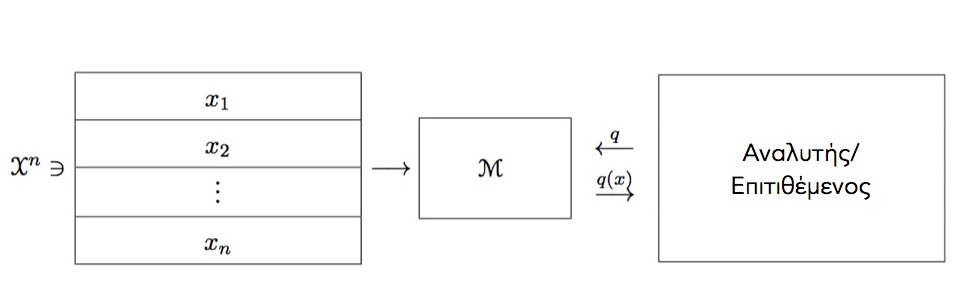
\includegraphics[scale=0.4]{images/M.jpg}
  \caption{Λειτουργία μηχανισμού ΔΙ}
  %\label{fig:boat1}
  \end{center}
\end{figure}



\subsection{Θεώρημα Σύνθεσης}

Στην εισαγωγή του κεφαλαίου αναφέραμε ότι η διαφορική ιδιωτικότητα χαρακτηρίζεται από δύο βασικές ιδιότητες. Αρχικά, εξασφαλίζει ότι τα αποτελέσματα θα είναι ανεπηρέαστα από οποιαδήποτε εξωτερική γνώση. Δεύτερον, η μέθοδος παρουσιάζει ανθεκτηκότητα στην μετεπεξεργασία. Όπως είδαμε, το αποτέλεσμα από την εφαρμογή ενός μηχανισμού ιδιωτικότητας κοινοποιείται, και εν συνεχεία αυτό μπορεί είτε να χρησιμοποιηθεί αυθαίρετα από άλλους είτε να χρησιμοποιηθεί ως δείγμα ώστε να εφαρμοστεί ένας νέομηχανισμός ακόμη και από τον ίδιο χρήστη. Η ανθεκτηκότητα στην επαναληπτική εφαρμογή μηχανισμών εγγυάται ότι δεν πρόκειται να χαθεί μέρος της ιδιωτικότητας, παρά την επαναχρησιμοποίηση\\
\textlatin{\cite{Dwork:2010:BDP:1917827.1918366}}.

\begin{theorem}\label{ak}(Σύνθεση)
 Έστω μηχανισμός $M:X\longrightarrow  B $ που παρέχει $\epsilon$-διαφορική ιδιωτικότητα. Τότε για κάθε συνάρτηση $f$, η σύνθεση $f\circ M$ διατηρεί $\epsilon$-διαφορική ιδιωτικότητα.
\end{theorem}

Στη συνέχεια εισάγουμε δυο κανόνες σύνθεσης που χρησιμοποιούνται συχνά για την δημιουργία νέων μηχανισμών ιδιωτικότητας. Ο νόμος της ακολουθιακής σύνθεσης παρουσιάζεται παρακάτω και χρησιμοποιείται συνήθως όταν απαιτείται ο υπολογισμός πολλών πληροφοριών από την ίδια βάση.


\begin{theorem} (Ακολουθιακή σύνθεση - \textlatin{sequential composition})\\
 Έστω μηχανισμός $M_1:X\longrightarrow  B $ που παρέχει $\epsilon_1$-διαφορική ιδιωτικότητα και μηχανισμός $M_2:X\longrightarrow  B $ που παρέχει $\epsilon_2$-διαφορική ιδιωτικότητα. Ορίζουμε νέο μηχανισμό $M(x)=(M_1(x),M_2(x))$, ο οποίος θα διατηρεί $(\epsilon_1+\epsilon_2)$-διαφορική ιδιωτικότητα.
\end{theorem}

Ας υποθέσουμε ότι έχουμε μια βάση δεδομένων με τους μισθούς μιας εταιρίας. Έστω ότι κάποιος θέλει να κοινοποιήσει την μέση τιμή, αλλά και την διακύμανση των μισθών. Θα χρησιμοποιήσει έναν μηχανισμό ιδιωτικότητας για τον μέσο και έναν για την διακύμανση, οι οποίοι στη συνέχεια μπορούν να συνδιαστούν δίνοντας την τάξη της ιδιωτικότητας που παρουσιάζεται στο θεώρημα. Τέλος, παρατηρούμε ότι το θεώρημα συνεπάγεται την εξής πρόταση:\textbf{ Όσο περισσότερες επερωτήσεις τίθενται στην ίδια βάση, τόσο περισσότερη ιδιωτικότητα χάνεται}.

Για συγκεκριμένες εφαρμογές που απαιτείται επαναχρησιμοποίηση, ο μηχανισμός που θα επιθυμούσαμε να σχεδιάσουμε είναι ένα αποτέλεσμα «προσαρμοστικής» σύνθεσης διάφορων μηχανισμών. Παρόμοια εφαρμόζονται και οι αλγορίθμοι μηχανικής μάθησης, όπου το αποτέλεσμα κάθε βήματος εξαρτάται απο τα προηγούμενα βήματα. Σε περιπτώσεις λοιπον που απαιτούνται επαναληπτικοί υπολογισμοί χρησιμοποιούμε αυτόν τον κανόνα για διατήρηση της ιδιωτικότητας:

\begin{theorem} (Προσαρμοστική σύνθεση - \textlatin{Adaptive composotion})\\
 Έστω μηχανισμός $M_1:X\longrightarrow  B_1 $ που παρέχει $\epsilon_1$-διαφορική ιδιωτικότητα και μηχανισμός $M_2:X\times B_1\longrightarrow  B_2 $ ώστε $M_2(\cdot, y_1)$ που παρέχει $\epsilon_2$-διαφορική ιδιωτικότητα για κάθε $y_1 \in B_1$. Ορίζουμε νέο μηχανισμό $M(x)=M_2(x,M_1(x))$, ο οποίος θα παρέχει $(\epsilon_1+\epsilon_2)$-διαφορική ιδιωτικότητα.
\end{theorem}

Ο κανόνας αυτός γενικεύει την έννοια της μετεπεξεργασίας που παρουσιάστηκε στο θεώρημα \ref{ak}, επειδή οποιαδήποτε συνάρτηση $f$ που δεν εξαρτάται από την βάση δεδομένων μπορεί να γίνει ένας μηχανισμός 0-διαφορικής ιδιωτικότητας. Επιλπέον αποτελεί γενίκευση και της ακολουθιακής σύνθεσης.

Τα παραπάνω θεωρήματα σύνθεσης ισχύουν και για τον γενικευμένο ορισμό της διαφορικής ιδιωτικότητας. Συγκεκριμένα, μετά την εφαρμογή της σύνθεσης σε μηχανισμούς που παρέχουν ($\epsilon_1, \delta_1$)-διαφορική ιδιωτικότητα και ($\epsilon_2, \delta_2$)-διαφορική ιδιωτικότητα, παρέχεται ($\epsilon_1+\epsilon_2, \delta_1+\delta_2$)-διαφορική ιδιωτικότητα. Παρακάτω παρουσιάζουμε ένα ακόμη θεώρημα σύνθεσης.

\begin{theorem} (Ανώτερη σύνθεση - \textlatin{Advanced composotion})\\
 Για κάθε $\epsilon, \delta, \delta'\geq 0$, ο μηχανισμός που δημιουργείται από την προσαρμοστική σύνθεση $k$ μηχανισμών με $(\epsilon, \delta)$-διαφορική ιδιωτικότητα, παρέχει $(\epsilon', k\delta+\delta')$-διαφορική ιδιωτικότητα me
 $$\epsilon'=\sqrt{2klog(1/\delta')} \epsilon+k\epsilon(e^\epsilon-1)$$
\end{theorem}
 Παρατηρούμε ότι όταν το $\epsilon$ είναι κοντά στο 0, τότε υπερισχύει ο πρώτος προσθετέος. 

Τα παραπάνω θεωρήματα σύνθεσης καλύπτουν τόσο την επαναληπτική εφαρμογή μηχανισμών διαφορικής ιδιωτικότητας στην ίδια βάση, όσο και την επαναληπτική εφαρμογή τους σε διαφορετικές βάσεις δεδομένων που όμως μπορεί να περιέχουν πληροφορίες σχετικές με μια συγκεκριμένη εγγραφή.









\clearpage
\section{Προσθήκη θορύβου και Μηχανισμοί}


Έστω $q$ μια επερώτηση τύπου \textlatin{counting query}. Προσπαθώντας να προστατέψουμε την ιδιωτικότητα με προσθήκη θορύβου προκύπτει η σχέση: 
$$M(x)=q(x)+noise$$

Πρέπει όμως να είμαστε προσεκτικοί στην ποσότητα θορύβου που θα προσθέσουμε. Η παρακάτω πρόταση περιγράφει επακριβώς τις δυο ακραίες καταστάσεις της σχέσης ποιότητας-ιδιωτικότητας: 

«Δημοσιεύοντας ένα σύνολο δεδομένων στο ακέραιο παρέχεται η καλύτερη δυνατή ποιότητα, ενώ με την πλήρη απόκρυψη παρέχεται η καλύτερη δυνατή ιδιωτικότητα.»

Δεδομένων συνόλων $x\sim x'$ μεγέθους $n$, παρατηρούμε ότι $|q(x)-q(x')|\leq 1/n$. Συμπεραίνουμε ότι θόρυβος μεγέθους $1/\epsilon n$ θα είναι αρκετός για να κάνει τις συναρτήσεις (μηχανισμούς) $M(x)$ και $M(x')$ «ε-πανομοιότυπες» με την έννοια που απαιτείται από τον ορισμό της διαφορικής ιδιωτικότητας. Έτσι, για κάθε αποτέλεσμα $y$ της επερώτησης $q$, πρέπει η κατανομή των απαντήσεων από τις $x$ και $x'$ να μοιάζει, κατά έναν παράγοντα της τάξης $e^\epsilon$. Αν $z$ είναι ο θόρυβος που προστείθεται, παρατηρούμε:
$$y=q(x)+z \Longleftrightarrow z=y-q(x)$$ και
$$y=q(x')+z' \Longleftrightarrow z'=y-q(x')$$
Προκύπτει $|z-z'|\leq 1/n$. Βλέπουμε ότι αρκεί η συνάρτηση κατανομής θορύβου να μεταβάλλεται κατά το πολύ $e^\epsilon$ σε διαστήματα μήκους $1/n$. Αυτό οδηγεί σε υιoθέτηση μοντέλων, όπως οι παρακάτω μηχανισμοί.


\subsection{Μηχανισμός \textlatin{Laplace}}
\begin{definition}(Κατανομή \textlatin{Laplace})\\
H κατανομή \textlatin{Laplace} με παράμετρο κλίμακας $b>0$ (θεωρώντας πάραμετρο θέσης 0) ορίζεται ως η κατανομή με συνάρτηση πυκνότητας πιθανότητας 
$$Lap(x|b)=\frac{1}{2b}e^{-\frac{|x|}{b}}$$
\end{definition}
Σημειώνεται ότι η διακύμανση της κατανομής είναι $\sigma^2=2b^2$ και η μέση τιμή $0$.

\begin{figure} [ht]
\begin{center}
  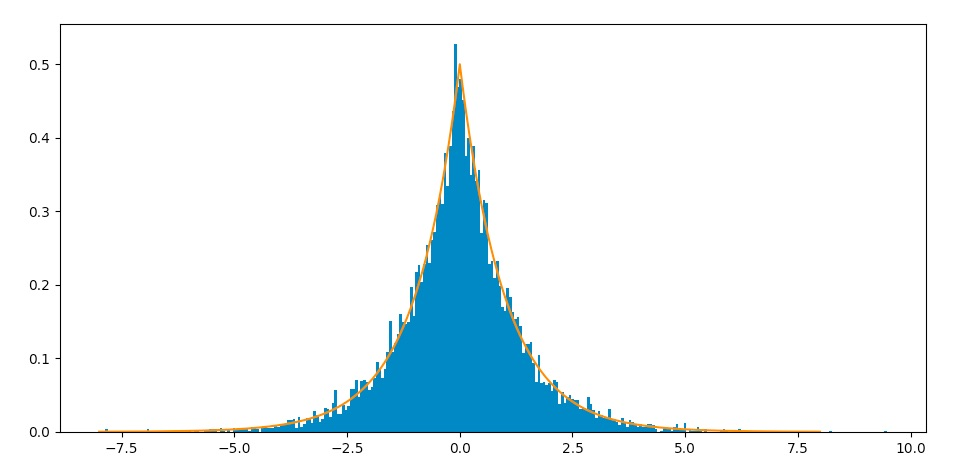
\includegraphics[scale=0.42]{images/Laplace1.jpg}
  \caption{Συνάρτηση πυκνότητας πιθανότητας κατανομής \textlatin{Laplace}, με παράμετρο κλίμακας $b=1$
}
  %\label{fig:boat1}
  \end{center}
\end{figure}


\begin{definition}(Ευαισθησία)\\
 Η $l_1$-ευαισθησία (\textlatin{sensitivity}) μιας συνάρτησης $f:X \longrightarrow \mathbb{R}^k$ είναι:
$$\Delta=max_{x\sim x'}||f(x)-f(x')||$$
\end{definition}
Η ευαισθησία μιάς επερώτησης $q$ καταγράφει το μέγεθος με το οποίο τα δεδομένα μιας και μόνο εγγραφής μπορούν να μεταβάλλουν την επερώτηση στην «χειρότερη» περίπτωση, και αντίστοιχα, τον θόρυβο που πρέπει να εισάγουμε στο αποτέλεσμα ώστε να αποκρύψουμε την συμμετοχή μιας εγγραφής στη βάση. 
Είναι προφανές ότι ένα \textlatin{counting query} έχει ευαισθησία $\Delta=1$.


\begin{theorem}(Μηχανισμός \textlatin{Laplace})\\
Έστω επερώτηση $q$ με σύνολο τιμών $\mathbb{R}$, και έστω $\Delta$ η $l_1$-ευαισθησία της. Τότε ο μηχανισμός 
$$M(x) = q(x) + z$$
με $z\sim Lap(\Delta|\epsilon)$, παρέχει $\epsilon$-διαφορική ιδιωτικότητα.
\end{theorem}

Το μέγεθος του θορύβου εξαρτάται από το είδος της επερώτησης και την επιλογή του $\epsilon$. Άρα για ένα \textlatin{counting query} θέλουμε θόρυβο τάξης $\sim Lap(1|\epsilon)$, ενώ όσο η τιμή του $\epsilon$ μικραίνει, τόσο το αποτέλεσμα γίνεται περισσότερο ανακριβές.

Θωρείστε την βάση δεδομένων $x$ με τους μισθούς που αναφέραμε προηγουμένως, και την επερώτηση για τον μέσο μισθό:
$$q(x)=\frac{\sum_{i=1}^{n}x_i}{n}$$
με $x_i\in [0,x_{max}]$. Αν χρησιμοποιήσουμε μια σχέση γειτνίασης τύπου $|x_i - x_i'|\leq x_{max}$ τότε η ευαισθησία της επερώτησης θα είναι 
$$\Delta=max_{x\sim x'}|q(x)-q(x')|=\frac{1}{n}max_{x_i,x'_i}|x_i - x'_i|\quad  i \in [1,n]$$ Έτσι έχουμε
$$\Delta=\frac{x_{max}}{n}$$
Σύμφωνα με το παραπάνω θεώρημα λοιπόν, ο μηχανισμός
$$M(x)=\frac{\sum_{i=1}^{n}x_i}{n}+Lap(\frac{x_{max}}{n\epsilon})$$
θα διατηρεί $\epsilon$-διαφορική ιδιωτικότητα.
Παρατηρούμε ότι το μέγεθος του θορύβου που προκύπτει από τον μηχανισμό \textlatin{Laplace} είναι αντιστρόφως ανάλογο του πλήθους $n$ των εγγραφών, πράγμα αναμενόμενο αφού διαισθητικά αναμένουμε καλύτερη ιδιωτικότητα αν το μέγεθος της βάσης είναι μεγάλο \textlatin{\cite{Corts2016DifferentialPI}}.

















\subsection{Εκθετικός Μηχανισμός}

Ενώ ο μηχανισμός \textlatin{Laplace} παρέχει διαφορική ιδιωτικότητα, δεν αρκεί για να καλύψει όλες τις ανάγκες, αφού εφαρμόζεται κυρίως σε επερωτήσεις που επιστρέφουν αριθμητικά αποτελέσματα. Μια χρήσιμη και αποτελεσματική μέθοδος για μη αριθμητικές επερωτήσεις είναι ο εκθετικός μηχανισμός \textlatin{\cite{dwork2008differential}}. Έδω απαιτείται η χρήση \textlatin{scoring} συναρτήσεων όπου αντιστοιχίζουν τα ζεύγη αποτελεσμάτων σε \textlatin{utility scores}. 

\begin{definition}(\textlatin{Scoring Function)}\\
Έστω $X$ το σύνολο όλων των πεπερασμένων συνόλων δεδομένων και $R$ το σύνολο τιμών ενός μηχανισμού $M$. Ως \textlatin{scoring} συνάρτηση ορίζεται:
$$u=X \times R \longrightarrow \mathbb{R}$$
και αποδίδει έναν βαθμό (\textlatin{score}) σε κάθε ζεύγος $(x,r)\in X \times R$.
 
\end{definition}
Όσο υψηλότερος είναι ο βαθμός του ζεύγους, τόσο καλύτερο το αποτέλεσμα. Η εφαρμογή που αποζητείται εδώ είναι να δίνεται μια βάση δεδομένων $x$ και ο μηχανισμός να επιστρέφει το $r\in R $ που μεγιστοποιεί τον βαθμό $u(x,r)$, ενώ παρέχει διαφορική ιδιωτικότητα.
%Παρ'όλο που η επιλογή της συνάρτησης μπορεί να γίνει αυθαιρέτως, υπάρχει συχνά φυσική επιλογή όταν η επερώτηση επιστρέφει το βέλτιστο αποτέλεσμα σε ένα πρόβλημα βελτιστοποίσης. 

Πριν παρουσιάσουμε τον εκθετικό μηχανισμό θα δώσουμε τον ορισμό της ευαισθησίας μιας \textlatin{scoring} συνάρτησης.

\begin{definition}
Η ευαισθησία μιας \textlatin{scoring} συνάρτησης $u=X \times R \longrightarrow \mathbb{R}$ είναι
\[ \Delta_u=\max_{r\in R} (\max_{x\sim x'}|u(x,r)-u(x',r)|)\]
\end{definition}

\begin{definition}(Εκθετικός Μηχανισμός)\\
Ως εκθετικός μηχανισμός ορίζεται μια τυχαιοποιημένη συνάρτηση $M_E:X\longrightarrow R$, η οποία δεδομένης βάσης $x\in X$ και παραμέτρου $\epsilon$, παράγει ένα στοιχείο $r\in R$ με πιθανότητα ανάλογη του $$ e^{\frac{e}{2\Delta_u}u(x,r)}$$
\end{definition}
Όπου $u$ είναι μια \textlatin{scoring} συνάρτηση και $\Delta_u$ η ευαισθησία της. O ορισμός συνεπάγεται το γεγονός ότι η πιθανότητα επιστροφής μιας τιμής $r$ αυξάνεται εκθετικά με την μεγιστοποίηση της τιμής $u(x,r)$. Η τιμή $r$ που μεγιστοποιεί την $u(x,r)$ έχει την μεγαλύτερη πιθανότητα.

\begin{theorem}
Ένας εκθετικός μηχανισμός παρέχει $\epsilon$-διαφορική ιδιωτικότητα.
\end{theorem}

Σε σύγκριση με τον μηχανισμό \textlatin{Laplace}, ο εκθετικός μηχανισμός είναι γενικότερος στο ότι δεν περιορίζει το ερώτημα να είναι αριθμητικό. Στην πράξη, ο εκθετικός μηχανισμός χρησιμοποιείται ευρύτερα σε περιπτώσεις όπου το σύνολο τιμών της επερώτησης είναι πεπερασμένο, έτσι ώστε η συνάρτηση πυκνότητας πιθανότητας να μπορεί να υπολογιστεί.



\subsection{Μηχανισμός \textlatin{Gauss}}

Εκτός από τον Μηχανισμό \textlatin{Laplace}, για την εφαρμογή ($\epsilon, \delta$)-διαφορικής ιδιωτικότητας σε αριθμητικές επερωτήσεις επιλέγεται και ο παρακάτω. Αρχικά δίνουμε τον ορισμό της $l2$ ευαισθησίας.

\begin{definition} 
 Η $l_2$-ευαισθησία (\textlatin{sensitivity}) μιας συνάρτησης $f:X \longrightarrow \mathbb{R}^k$ είναι:
$$\Delta_2=max_{x\sim x'}||f(x)-f(x')||_2$$
\end{definition}

Υπενθυμίζουμε την λειτουργία της ευκλείδιας νόρμας: $||x||_2=\sqrt{x_1^2+x_2^2+...+x_n^2}$

\begin{theorem}
Έστω επερώτηση $q$ με σύνολο τιμών $\mathbb{R}$ και $\Delta_2$ ευαισθησία. Για $\epsilon>0$ και $\delta>0$ ο μηχανισμός
$$M(x) = q(x) + z$$
με $z$ ένα τυχαίο διάνυσμα ανεξάρτηων τυχαίων μεταβλητών που ακολουθούν την Κανονική κατανομή με μέση τιμή 0 και διακύμανση $\sigma^2=c^2\Delta^2_2$, me $c=\sqrt{2log(1.25/\delta}/\epsilon$, παρέχει $(\epsilon, \delta)$- διαφορική ιδιωτικότητα.

\end{theorem}

 Δεν προκαλεί έκπληξη το γεγονός ότι εμφανίζεται ο όρος δ: η κατανομή \textlatin{Laplace} είναι ιδανική για πολλαπλασιαστικό φράγμα, αλλά η Κανονική κατανομή όχι.  Αν βέβαια το $\delta$ είναι επαρκώς (π.χ. λογαριθμικά) μικρό, στην πράξη δεν θα βιώσουμε ποτέ αδυναμία εγγύησης της ιδιωτικότητας. 
 
 Επίσης, ένα να απο τα πλεονεκτήματα αυτού του μηχανισμού είναι ότι το άθροισμα δυο μηχανισμών $\textlatin{Gauss}$ είναι μηχανιμός $\textlatin{Gauss}$, πράγμα που κάνει ευκολότερη την κατανόηση της εφαρμογής του κατά την ανάλυση δεδομένων. 
Οι δύο μηχανισμοί δίνουν την ίδια απώλεια αθροιστικά κατά τη σύνθεση, οπότε αν και η εγγύηση απορρήτου είναι ασθενέστερη για κάθε μεμονωμένο υπολογισμό, τα αθροιστικά αποτελέσματα μετά από πολλούς υπολογισμούς είναι ανταγωνιστικά. Τελικά προκύπτει ότι η χρήση του μηχανισμού \textlatin{Laplace} είναι καθαρότερη, ενώ οι δύο μηχανισμοί συμπεριφέρονται παρόμοια σε περιπτώσεις σύνθεσης \textlatin{\cite{Dwork:2010:BDP:1917827.1918366}}.


%Σκεφτείτε το Report Noisy Max (με τον θόρυβο Laplace) σε μια περίπτωση όπου κάθε υποψήφια παραγωγή έχει την ίδια βαθμολογία ποιότητας στη βάση δεδομένων x και στη γειτονική γ. Ανεξάρτητα από τον αριθμό των υποψηφίων αποτελεσμάτων, ο μηχανισμός αποδίδει (ε, 0) -διαπροσωπευτική ιδιωτικότητα

\section{Κατασκευή σύνθετων Μηχανισμών}

Οι μηχανισμοί που παρουσιάστηκαν παραπάνω είναι αρκετά γενικοί και απλοί στην εφαρμογή. Όπως θα δούμε και στη συνέχεια, η μόνη ποσότητα που χρειάζεται να υπολογιστεί για την υλοποίηση αυτών των αλγορίθμων είναι η ευαισθησία. Παρόλο που συνήθως υπολογίζεται εύκολα για απλές επερωτήσεις, μπορεί να είναι δύσκολο να υπολογιστεί για περίπλοκα ερωτήματα (π.χ., η βέλτιστη λύση ενός προβλήματος μη γραμμικής βελτιστοποίησης). Όταν οι επερωτήσεις είναι περίπλοκες, μια κοινή στρατηγική είναι η αποδόμηση της υπο έρευνα επερώτησης έτσι ώστε η ευαισθησία κάθε μέρους της να μπορεί εύκολα να υπολογιστεί.
Παραδείγματος χάριν, αν και η ευαισθησία της βέλτιστης λύσης ενός προβλήματος μη γραμμικής βελτιστοποίησης μπορεί να μην είναι εύκολο να υπολογιστεί, η ευαισθησία των ενδιάμεσων αποτελεσμάτων που χρησιμοποιούνται για να υπολογιστεί επαναληπτικά η βέλτιστη λύση είναι συχνά πιο απλό να υπολογιστεί. Έτσι, χρησιμοποιώντας τους κανόνες σύνθεσης, μπορεί κανείς να κατασκευάσει τον επιθυμητό μηχανισμό ιδιωτικότητας.


Τολμούμε να πούμε ότι η Διαφορική Ιδιωτικότητα αποτελεί την «ασφαλέστερη» επιλογή από τους μηχανισμούς προστασίας που αναλύσαμε. Ο κύριος λόγος είναι ότι η εφαρμογή της δεν επηρεάζεται από την γνώση που κατέχει ο επιτιθέμενος. Επιπλέον, λόγω αυτού, δεν υπάρχει και η ανάγκη μοντελοποίησης της πρότερης γνώσης, οδηγώντας σε ελαφρώς ταχύτερους αλγορίθμους. 


Στην πραγματικότητα, η Διαφορική Ιδιωτικότητα υπόσχεται να προστατεύει τα άτομα από κάθε πιθανή απειλή που θα μπορούσαν να αντιμετωπίσουν λόγω της ύπαρξης των δεδομένων τους στην ιδιωτική βάση δεδομένων $x$ και που δεν θα αντιμετόπιζαν εάν τα δεδομένα τους δεν ήταν μέρος της $x$. Παρόλο που οι εγγραφές μπορούν πράγματι να απειληθούν μόλις απελευθερωθούν τα αποτελέσματα ενός μηχανισμού ΔΙ, η διαφορική ιδιωτικότητα υπόσχεται ότι η πιθανότητα διαρροής δεν αυξάνεται σημαντικά από την επιλογή συμμετοχής τους.
Κατά κάποιο τρόπο αξιολογείται η απόφαση ενός ατόμου αν θα συμπεριλάβει ή όχι τα δεδομένα του σε μια βάση δεδομένων που θα χρησιμοποιηθεί ένας μηχανισμός ΔΙ. Εξετάζεται η διαφορά δηλαδή μεταξύ
της πιθανότητας διαρροής δεδομένου ότι συμμετέχει στη βάση, σε σύγκριση με την πιθανότητα διαρροής δεδομένου ότι δεν συμμετέχει.




